\documentclass[11pt,letterpaper]{article}
\usepackage[margin=.65in,headheight=16pt,headsep=16pt,footskip=22pt]{geometry}
\usepackage[T1]{fontenc}
\usepackage{helvet}
\renewcommand{\familydefault}{\sfdefault}
\usepackage{tikz}
\usetikzlibrary{arrows.meta,calc}
\usepackage{array,tabularx,fancyhdr,amsmath}
\pagestyle{fancy}\fancyhf{}
\newcommand{\band}{Grades 2--5}
\fancyhead[L]{\small Week 56 / Corners of a solid / \band}
\fancyfoot[L]{\scriptsize Bellingham Math Circle / Week 56 / N56-S-v2}
\fancyfoot[R]{\scriptsize\thepage}
\renewcommand{\headrulewidth}{.35pt}\renewcommand{\footrulewidth}{.25pt}
\setlength{\parindent}{0pt}\setlength{\parskip}{7pt}
\newcommand{\problem}[2]{\noindent\textbf{Problem #1:} #2\par}
\newcommand{\blank}[1]{\vspace{#1}}
\newcommand{\workbox}[1]{\begin{tikzpicture}\draw[gray!50,rounded corners=2pt] (0,0) rectangle (17.8,#1);\end{tikzpicture}}
\newcommand{\cube}[1][]{\begin{tikzpicture}[x=.55cm,y=.55cm,#1]
 \coordinate (A) at (0,0);\coordinate (B) at (2.2,0);\coordinate (C) at (2.2,2.2);\coordinate (D) at (0,2.2);
 \coordinate (E) at (.8,.7);\coordinate (F) at (3,.7);\coordinate (G) at (3,2.9);\coordinate (H) at (.8,2.9);
 \fill[blue!10] (A)--(B)--(C)--(D)--cycle;\fill[blue!5] (D)--(C)--(G)--(H)--cycle;\fill[blue!17] (B)--(F)--(G)--(C)--cycle;
 \draw (A)--(B)--(C)--(D)--cycle (D)--(H)--(G)--(F)--(B) (C)--(G);
 \draw[dashed,gray] (A)--(E)--(F) (E)--(H);
 \end{tikzpicture}}
\newcommand{\tetra}{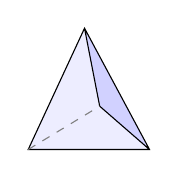
\begin{tikzpicture}[x=.55cm,y=.55cm]
 \fill[blue!7] (0,0)--(2.8,0)--(1.3,2.8)--cycle;
 \fill[blue!18] (2.8,0)--(1.65,1)--(1.3,2.8)--cycle;
 \draw (0,0)--(2.8,0)--(1.3,2.8)--cycle (2.8,0)--(1.65,1)--(1.3,2.8);
 \draw[dashed,gray] (0,0)--(1.65,1);
 \end{tikzpicture}}
\newcommand{\octa}{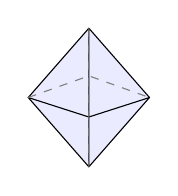
\begin{tikzpicture}[x=.55cm,y=.55cm]
 \fill[blue!8] (0,1.6)--(1.4,3.2)--(2.8,1.6)--(1.4,0)--cycle;
 \draw (0,1.6)--(1.4,3.2)--(2.8,1.6)--(1.4,0)--cycle (1.4,3.2)--(1.4,1.15)--(1.4,0) (0,1.6)--(1.4,1.15)--(2.8,1.6);
 \draw[dashed,gray] (1.4,3.2)--(1.4,2.1)--(1.4,0) (0,1.6)--(1.4,2.1)--(2.8,1.6);
 \end{tikzpicture}}
\newcommand{\prism}{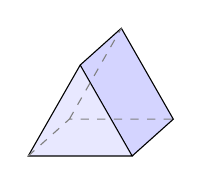
\begin{tikzpicture}[x=.55cm,y=.55cm]
 \fill[blue!9] (0,0)--(2.4,0)--(1.2,2.1)--cycle;
 \fill[blue!17] (2.4,0)--(3.35,.85)--(2.15,2.95)--(1.2,2.1)--cycle;
 \draw (0,0)--(2.4,0)--(1.2,2.1)--cycle (2.4,0)--(3.35,.85)--(2.15,2.95)--(1.2,2.1);
 \draw[dashed,gray] (0,0)--(.95,.85)--(3.35,.85) (.95,.85)--(2.15,2.95);
 \end{tikzpicture}}
\newcommand{\pyramid}{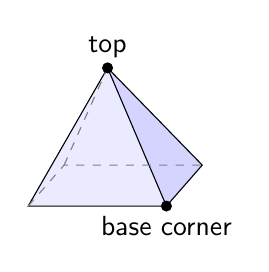
\begin{tikzpicture}[x=.65cm,y=.65cm]
 \fill[blue!8] (0,0)--(2.7,0)--(1.55,2.7)--cycle;
 \fill[blue!17] (2.7,0)--(3.4,.8)--(1.55,2.7)--cycle;
 \draw (0,0)--(2.7,0)--(3.4,.8)--(1.55,2.7)--cycle (2.7,0)--(1.55,2.7);
 \draw[dashed,gray] (0,0)--(.7,.8)--(3.4,.8) (.7,.8)--(1.55,2.7);
 \fill (1.55,2.7) circle (2pt);\node[above] at (1.55,2.7) {top};
 \fill (2.7,0) circle (2pt);\node[below] at (2.7,0) {base corner};
 \end{tikzpicture}}
\newcommand{\circleblank}[1]{\begin{tikzpicture}[x=1cm,y=1cm]
 \draw[gray!60] (0,0) circle (1.9);\fill (0,0) circle (1.4pt);\node[below] at (0,-2.05) {#1};\end{tikzpicture}}
\newcommand{\turnexample}{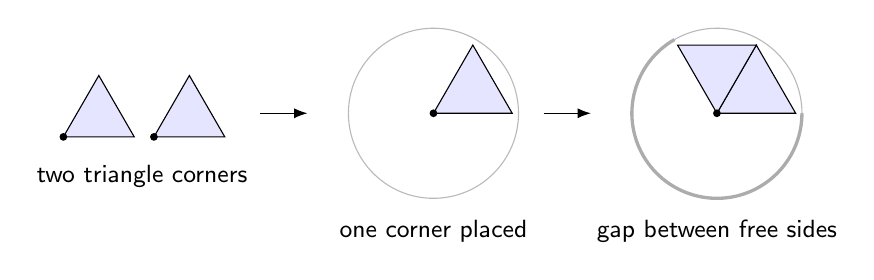
\begin{tikzpicture}[x=1cm,y=1cm,font=\small]
 \draw[fill=blue!10] (-.8,0)--(.1,0)--(-.35,.7794)--cycle;
 \draw[fill=blue!10] (.35,0)--(1.25,0)--(.8,.7794)--cycle;
 \fill (-.8,0) circle (1.4pt);\fill (.35,0) circle (1.4pt);
 \node at (.2,-.5) {two triangle corners};
 \draw[-{Latex}] (1.7,.3)--(2.3,.3);
 \begin{scope}[shift={(3.9,.3)}]
  \draw[gray!55] (0,0) circle (1.08);
  \draw[fill=blue!10] (0,0)--(1,0)--(.5,.866)--cycle;
  \fill (0,0) circle (1.4pt);\node at (0,-1.5) {one corner placed};
 \end{scope}
 \draw[-{Latex}] (5.3,.3)--(5.9,.3);
 \begin{scope}[shift={(7.5,.3)}]
  \draw[gray!55] (0,0) circle (1.08);
  \draw[fill=blue!10] (0,0)--(1,0)--(.5,.866)--cycle;
  \draw[fill=blue!10] (0,0)--(.5,.866)--(-.5,.866)--cycle;
  \draw[very thick,gray!65] (120:1.08) arc (120:360:1.08);
  \fill (0,0) circle (1.4pt);\node at (0,-1.5) {gap between free sides};
 \end{scope}
\end{tikzpicture}}

\begin{document}
Use closed models with all their faces attached. A vertex is a corner of the assembled solid; an edge is shared by two faces. Count each assembled edge and vertex once. Tabs and glue overlaps do not count.

\begin{center}
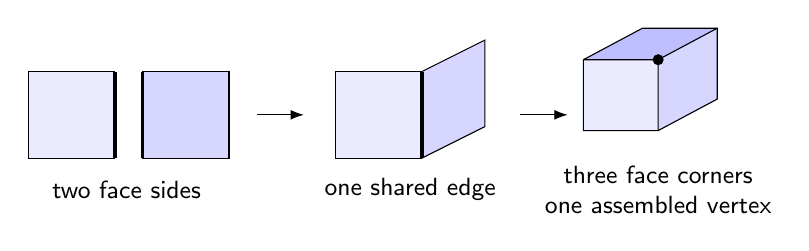
\begin{tikzpicture}[x=1cm,y=1cm,font=\small]
 \draw[fill=blue!8] (0,0) rectangle (1.1,1.1);
 \draw[fill=blue!16] (1.45,0) rectangle (2.55,1.1);
 \draw[very thick] (1.1,0)--(1.1,1.1) (1.45,0)--(1.45,1.1);
 \node at (1.25,-.4) {two face sides};
 \draw[-{Latex}] (2.9,.55)--(3.5,.55);
 \draw[fill=blue!8] (3.9,0) rectangle (5,1.1);
 \draw[fill=blue!16] (5,0)--(5.8,.4)--(5.8,1.5)--(5,1.1)--cycle;
 \draw[very thick] (5,0)--(5,1.1);
 \node at (4.85,-.4) {one shared edge};
 \draw[-{Latex}] (6.25,.55)--(6.85,.55);
 \begin{scope}[shift={(8,.35)}]
  \fill[blue!8] (0,0)--(-.95,0)--(-.95,.9)--(0,.9)--cycle;
  \fill[blue!16] (0,0)--(.75,.4)--(.75,1.3)--(0,.9)--cycle;
  \fill[blue!25] (0,.9)--(-.95,.9)--(-.2,1.3)--(.75,1.3)--cycle;
  \draw (0,0)--(-.95,0)--(-.95,.9)--(-.2,1.3)--(.75,1.3)--(.75,.4)--cycle;
  \draw (-.95,.9)--(0,.9)--(.75,1.3) (0,0)--(0,.9);
  \fill (0,.9) circle (2pt);
 \end{scope}
 \node[align=center] at (8,-.4) {three face corners\\one assembled vertex};
\end{tikzpicture}
\end{center}

\problem{1}{Find the vertices, edges and faces of each closed model.}
\begin{center}
\renewcommand{\arraystretch}{1.1}
\begin{tabular}{|>{\centering\arraybackslash}m{5.4cm}|>{\centering\arraybackslash}m{3.0cm}|>{\centering\arraybackslash}m{3.0cm}|>{\centering\arraybackslash}m{3.0cm}|}
\hline Model & Vertices $V$ & Edges $E$ & Faces $F$\\\hline
\cube\ \small cube & & & \\[5pt]\hline
\tetra\ \small tetrahedron & & & \\[5pt]\hline
\prism\ \small triangular prism & & & \\[5pt]\hline
\octa\ \small octahedron & & & \\[5pt]\hline
\end{tabular}
\end{center}

\newpage
\problem{2}{Imagine cutting every face free. Find a rule that turns the number of separate face sides into the assembled edge count. Can the separate face-corner count alone tell you the vertex count?}

\begin{center}
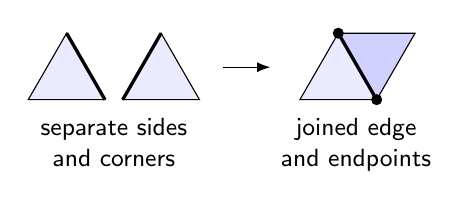
\begin{tikzpicture}[x=.75cm,y=.75cm,font=\small]
 \draw[fill=blue!8] (0,0)--(1.3,0)--(.65,1.1258)--cycle;
 \draw[fill=blue!8] (1.6,0)--(2.9,0)--(2.25,1.1258)--cycle;
 \draw[very thick] (1.3,0)--(.65,1.1258) (1.6,0)--(2.25,1.1258);
 \node[below,align=center] at (1.45,-.15) {separate sides\\and corners};
 \draw[-{Latex}] (3.3,.55)--(4.1,.55);
 \draw[fill=blue!8] (4.6,0)--(5.9,0)--(5.25,1.1258)--cycle;
 \draw[fill=blue!18] (5.9,0)--(6.55,1.1258)--(5.25,1.1258)--cycle;
 \draw[very thick] (5.9,0)--(5.25,1.1258);\fill (5.9,0) circle (2pt);\fill (5.25,1.1258) circle (2pt);
 \node[below,align=center] at (5.55,-.15) {joined edge\\and endpoints};
\end{tikzpicture}
\end{center}

\begin{center}\renewcommand{\arraystretch}{1.1}
\begin{tabular}{|m{4.7cm}|>{\centering\arraybackslash}m{2.6cm}|>{\centering\arraybackslash}m{2.6cm}|>{\centering\arraybackslash}m{2.6cm}|>{\centering\arraybackslash}m{2.6cm}|}
\hline Faces before assembly & Separate sides & Assembled edges & Separate corners & Assembled vertices\\\hline
6 squares: cube &&&&\\[36pt]\hline
4 triangles: tetrahedron &&&&\\[36pt]\hline
2 triangles and 3 squares: prism &&&&\\[36pt]\hline
8 triangles: octahedron &&&&\\[36pt]\hline
\end{tabular}\end{center}
\blank{.2cm}\workbox{4.9}

\newpage
Join face corners around one point. Keep their sides meeting edge to edge and their marked vertices together. The gap is the missing part of a full turn when the corners lie flat.
\begin{center}\turnexample\end{center}
\problem{3}{Which groups can close into a pointed corner with no inward dents? Which close flat with no gap? Make each group, then draw its gap with the corners laid flat.}
\begin{center}
\circleblank{3 triangles}\hspace{.7cm}\circleblank{4 triangles}\hspace{.7cm}\circleblank{5 triangles}
\par\vspace{.5cm}
\circleblank{6 triangles}\hspace{.7cm}\circleblank{3 squares}\hspace{.7cm}\circleblank{4 squares}
\end{center}
\blank{.35cm}\workbox{3.4}

\newpage
A full turn is $360^\circ$. An equilateral triangle corner is $60^\circ$; a square corner is $90^\circ$. A vertex's gap is $360^\circ$ minus its face-corner angles.

\begin{center}
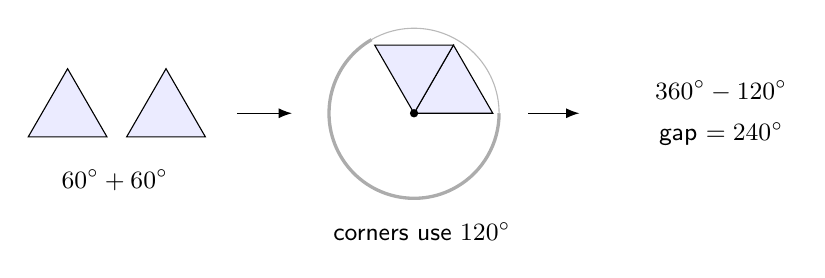
\begin{tikzpicture}[x=1cm,y=1cm,font=\small]
 \draw[fill=blue!8] (-.8,0)--(.2,0)--(-.3,.866)--cycle;
 \draw[fill=blue!8] (.45,0)--(1.45,0)--(.95,.866)--cycle;
 \node at (.3,-.55) {$60^\circ+60^\circ$};
 \draw[-{Latex}] (1.85,.3)--(2.55,.3);
 \begin{scope}[shift={(4.1,.3)}]
  \draw[gray!55] (0,0) circle (1.08);
  \draw[fill=blue!8] (0,0)--(1,0)--(.5,.866)--cycle;
  \draw[fill=blue!8] (0,0)--(.5,.866)--(-.5,.866)--cycle;
  \draw[very thick,gray!65] (120:1.08) arc (120:360:1.08);
  \fill (0,0) circle (1.5pt);\node at (.1,-1.5) {corners use $120^\circ$};
 \end{scope}
 \draw[-{Latex}] (5.55,.3)--(6.2,.3);
 \node[align=center] at (8,.3) {$360^\circ-120^\circ$\\[4pt]gap $=240^\circ$};
\end{tikzpicture}
\end{center}

\problem{4}{Find the gap at every vertex of each closed model. How many full turns do all its gaps make together?}
\begin{center}\renewcommand{\arraystretch}{1.1}
\begin{tabular}{|m{3.1cm}|>{\centering\arraybackslash}m{2.6cm}|>{\centering\arraybackslash}m{3.6cm}|>{\centering\arraybackslash}m{2.7cm}|>{\centering\arraybackslash}m{3.2cm}|}
\hline Model & Vertices & Face corners at one vertex & Gap at one vertex & All gaps together\\\hline
Cube &&&&\\[43pt]\hline
Tetrahedron &&&&\\[43pt]\hline
Triangular prism &&&&\\[43pt]\hline
Octahedron &&&&\\[43pt]\hline
\end{tabular}\end{center}
\blank{.15cm}\workbox{4.2}

\newpage
\problem{5}{The square pyramid has one square face and four equilateral triangle faces. Find its total gap.}
\begin{center}\pyramid\hspace{1.2cm}
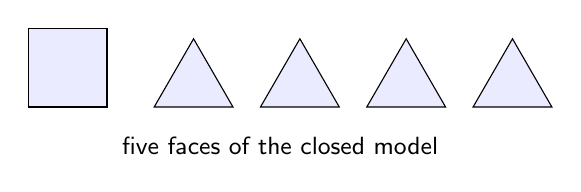
\begin{tikzpicture}[x=1cm,y=1cm,font=\small]
 \draw[fill=blue!8] (0,0) rectangle (1,1);
 \foreach \x in {1.6,2.95,4.3,5.65}{\draw[fill=blue!8] (\x,0)--++(1,0)--++(-.5,.866)--cycle;}
 \node at (3.2,-.5) {five faces of the closed model};
\end{tikzpicture}\end{center}
\begin{center}\renewcommand{\arraystretch}{1.15}
\begin{tabular}{|m{4.0cm}|>{\centering\arraybackslash}m{3.1cm}|>{\centering\arraybackslash}m{4.1cm}|>{\centering\arraybackslash}m{3.7cm}|}
\hline Vertex type & How many? & Face corners meeting there & Gap at each one\\\hline
Top &&&\\[55pt]\hline
Base corner &&&\\[55pt]\hline
\end{tabular}\end{center}
\blank{.6cm}\workbox{9.3}

\newpage
In a redrawn surface, marked points count as vertices, segments between vertices count as edges, and each face piece counts as a face.

\problem{6}{Compare $V-E+F$ for all four models in Problem 1. Keep the cube's shape and try these three changes to its surface drawing. What happens to $V-E+F$ and to the total gap? Can a new vertex have a gap while the cube keeps its shape?}
\begin{center}
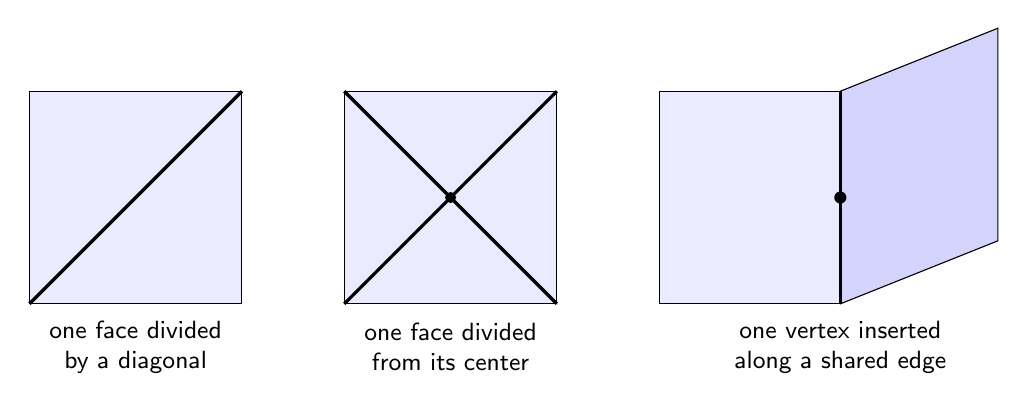
\begin{tikzpicture}[x=1cm,y=1cm,font=\small]
 \draw[fill=blue!8] (0,0) rectangle (2.7,2.7);\draw[very thick] (0,0)--(2.7,2.7);
 \node[align=center] at (1.35,-.55) {one face divided\\by a diagonal};
 \draw[fill=blue!8] (4,0) rectangle (6.7,2.7);
 \foreach \p in {(4,0),(6.7,0),(6.7,2.7),(4,2.7)}{\draw[very thick] \p --(5.35,1.35);}
 \fill (5.35,1.35) circle (2pt);\node[align=center] at (5.35,-.55) {one face divided\\from its center};
 \draw[fill=blue!8] (8,0) rectangle (10.3,2.7);
 \draw[fill=blue!17] (10.3,0)--(12.3,.8)--(12.3,3.5)--(10.3,2.7)--cycle;
 \draw[very thick] (10.3,0)--(10.3,2.7);\fill (10.3,1.35) circle (2.2pt);
 \node[align=center] at (10.3,-.55) {one vertex inserted\\along a shared edge};
\end{tikzpicture}\end{center}
\begin{center}\renewcommand{\arraystretch}{1.15}
\begin{tabular}{|m{3.3cm}|>{\centering\arraybackslash}m{2cm}|>{\centering\arraybackslash}m{2cm}|>{\centering\arraybackslash}m{2cm}|>{\centering\arraybackslash}m{2.7cm}|>{\centering\arraybackslash}m{3.1cm}|}
\hline Closed surface & $V$ & $E$ & $F$ & $V-E+F$ & Total gap\\\hline
Original cube &&&&&\\[25pt]\hline
One diagonal &&&&&\\[25pt]\hline
Center and 4 lines &&&&&\\[25pt]\hline
One edge vertex &&&&&\\[25pt]\hline
\end{tabular}\end{center}
\blank{.3cm}\workbox{6.0}

\newpage\renewcommand{\band}{Grades 4--5}
Convex means no dents. An opened drawing preserves the assembled edge and vertex connections. Count its bounded regions as faces; the outside is the removed face. A tree is a connected drawing with no closed loops.

\begin{center}
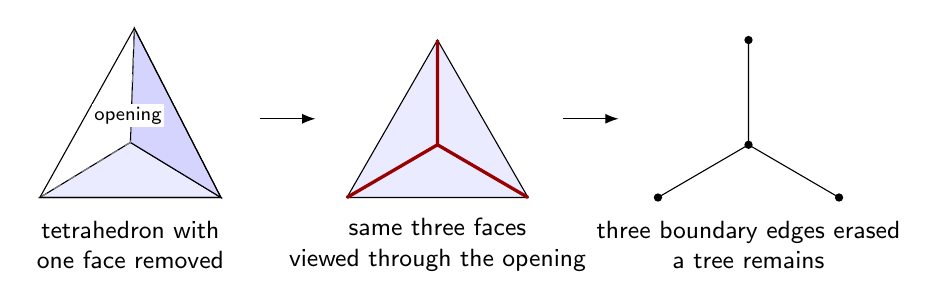
\begin{tikzpicture}[x=1cm,y=1cm,font=\small]
 \draw[fill=blue!8] (0,0)--(2.3,0)--(1.15,.7)--cycle;
 \draw[fill=blue!17] (2.3,0)--(1.15,.7)--(1.2,2.15)--cycle;
 \draw[dashed,gray] (0,0)--(1.15,.7)--(1.2,2.15);
 \draw (0,0)--(2.3,0)--(1.2,2.15)--cycle;
 \node[font=\scriptsize,fill=white,inner sep=1pt] at (1.12,1.04) {opening};
 \node[align=center] at (1.15,-.6) {tetrahedron with\\one face removed};
 \draw[-{Latex}] (2.8,1)--(3.5,1);
 \draw[fill=blue!8] (3.9,0)--(6.2,0)--(5.05,2)--cycle;
 \draw[very thick,red!60!black] (3.9,0)--(5.05,.67)--(6.2,0) (5.05,.67)--(5.05,2);
 \node[align=center] at (5.05,-.6) {same three faces\\viewed through the opening};
 \draw[-{Latex}] (6.65,1)--(7.35,1);
 \draw (7.85,0)--(9.0,.67)--(10.15,0) (9.0,.67)--(9.0,2);
 \foreach \p in {(7.85,0),(9.0,.67),(10.15,0),(9.0,2)}{\fill \p circle (1.5pt);}
 \node[align=center] at (9,-.6) {three boundary edges erased\\a tree remains};
\end{tikzpicture}\end{center}

\problem{7}{Explain why $V-E+F$ always has the same value for closed convex solids with polygon faces. Can an opened drawing be changed into a tree while keeping all its vertices connected?}

\begin{center}
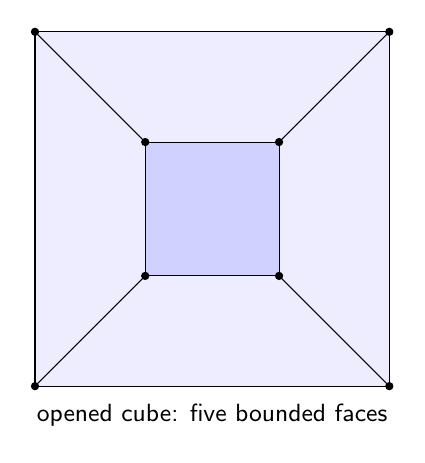
\begin{tikzpicture}[x=1cm,y=1cm,font=\small]
 \draw[fill=blue!7] (0,0) rectangle (4.5,4.5);\draw[fill=blue!18] (1.4,1.4) rectangle (3.1,3.1);
 \draw (0,0)--(1.4,1.4) (4.5,0)--(3.1,1.4) (4.5,4.5)--(3.1,3.1) (0,4.5)--(1.4,3.1);
 \foreach \p in {(0,0),(4.5,0),(4.5,4.5),(0,4.5),(1.4,1.4),(3.1,1.4),(3.1,3.1),(1.4,3.1)}{\fill \p circle (1.5pt);}
 \node[below] at (2.25,-.1) {opened cube: five bounded faces};
\end{tikzpicture}\hspace{.7cm}
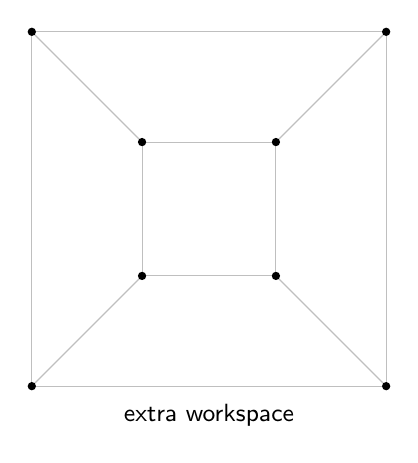
\begin{tikzpicture}[x=1cm,y=1cm,font=\small]
 \draw[gray!50] (0,0) rectangle (4.5,4.5);\draw[gray!50] (1.4,1.4) rectangle (3.1,3.1);
 \draw[gray!50] (0,0)--(1.4,1.4) (4.5,0)--(3.1,1.4) (4.5,4.5)--(3.1,3.1) (0,4.5)--(1.4,3.1);
 \foreach \p in {(0,0),(4.5,0),(4.5,4.5),(0,4.5),(1.4,1.4),(3.1,1.4),(3.1,3.1),(1.4,3.1)}{\fill \p circle (1.5pt);}
 \node[below] at (2.25,-.1) {extra workspace};
\end{tikzpicture}\end{center}
\blank{.3cm}\workbox{6.8}

\newpage
The angles of a triangle add to $180^\circ$. A polygon with $n$ sides can be divided into $n-2$ triangles, so its corner angles add to $180(n-2)^\circ$.
\begin{center}
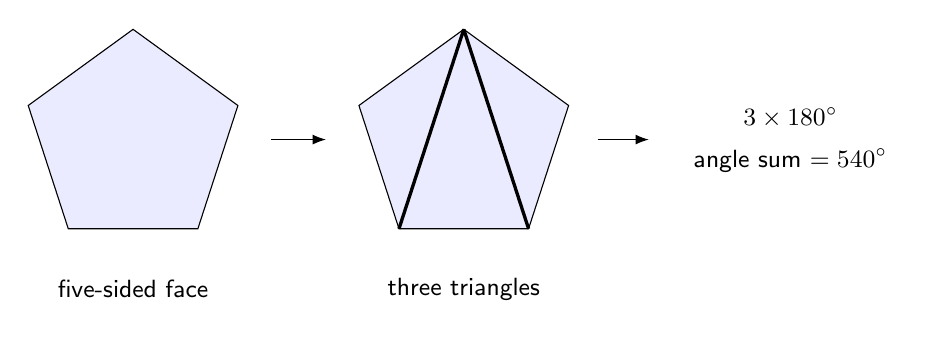
\begin{tikzpicture}[x=1cm,y=1cm,font=\small]
 \foreach \s/\x in {0/0,1/4.2}{
  \begin{scope}[shift={(\x,0)}]
   \foreach \i in {0,...,4}{\coordinate (P\i) at (90+72*\i:1.4);}
   \draw[fill=blue!8] (P0)--(P1)--(P2)--(P3)--(P4)--cycle;
   \ifnum\s=1\draw[very thick] (P0)--(P2) (P0)--(P3);\fi
  \end{scope}
 }
 \node at (0,-1.9) {five-sided face};\node at (4.2,-1.9) {three triangles};
 \draw[-{Latex}] (1.75,0)--(2.45,0);\draw[-{Latex}] (5.9,0)--(6.55,0);
 \node[align=center] at (8.35,0) {$3\times180^\circ$\\[4pt]angle sum $=540^\circ$};
\end{tikzpicture}\end{center}

\problem{8}{Explain why every closed convex solid with polygon faces has the same total gap, even when its vertex gaps are different.}
\blank{.3cm}\workbox{14.5}

\newpage
A regular polygon has equal sides and equal angles. Every face of each solid below is one regular polygon.

\problem{9}{Find the number of vertices, edges and faces each closed convex solid with polygon faces must have, without a model of the whole solid.}

\begin{center}
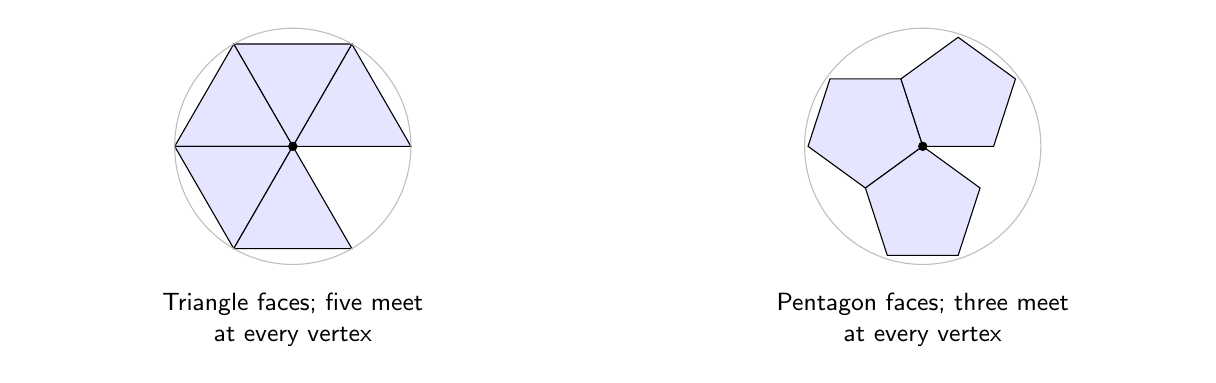
\begin{tikzpicture}[x=1cm,y=1cm,font=\small]
 \begin{scope}[shift={(0,0)}]
  \foreach \a in {0,60,120,180,240}{\draw[fill=blue!10] (0,0)--(\a:1.5)--(\a+60:1.5)--cycle;}
  \draw[gray!50] (0,0) circle (1.5);\fill (0,0) circle (1.7pt);
  \node[align=center,text width=6.5cm] at (0,-2.2) {Triangle faces; five meet\\at every vertex};
 \end{scope}
 \begin{scope}[shift={(8,0)}]
  \foreach \a in {0,108,216}{\begin{scope}[rotate=\a]
   \draw[fill=blue!10] (0,0)--(.9,0)--(1.178115,.855951)--(.45,1.384957)--(-.278115,.855951)--cycle;
  \end{scope}}
  \draw[gray!50] (0,0) circle (1.5);\fill (0,0) circle (1.7pt);
  \node[align=center,text width=6.5cm] at (0,-2.2) {Pentagon faces; three meet\\at every vertex};
 \end{scope}
\end{tikzpicture}\end{center}
\begin{center}\renewcommand{\arraystretch}{1.2}
\begin{tabular}{|m{5.5cm}|>{\centering\arraybackslash}m{3.1cm}|>{\centering\arraybackslash}m{3.1cm}|>{\centering\arraybackslash}m{3.1cm}|}
\hline Solid & Vertices & Edges & Faces\\\hline
Five triangles at each vertex &&&\\[35pt]\hline
Three pentagons at each vertex &&&\\[35pt]\hline
\end{tabular}\end{center}
\blank{.35cm}\workbox{9.0}
\end{document}
